\section{3D-Modell}
Das nächste Ziel besteht darin ein Regelungskonzept zu entwickeln, welches das Balancieren des Würfels auf einer Ecke ermöglicht. Hierfür werden drei Motor verwendet, wodurch das gesamte System über sechs Freiheitsgrade verfügt. Die Vorgehensweise erfolgt analog zu dem Reglerentwurf der Würfelseite. Somit besteht der erste Schritt in dem Entwurf eines mechanischen Modells, welches wiederum zu einer Zustandsraumdarstellung führt, die als Grundlage für den Reglerentwurf verwendet wird.
Zu Beginn dieses Kapitels werden die Systemparameter vorgestellt, deren Bestimmung diskutiert und erste Annahmen getroffen um die weitere Modellbildung zu vereinfachen. Im zweiten Abschnitt wird die Kinematik des Systems untersucht. Hierbei werden zunächst die nötigen Bezugssysteme und generalisierten Koordinaten definiert, die anschließend für die Bestimmung der generalisierten und partiellen Geschwindigkeiten benötigt werden.
Der nächste Abschnitt widmet sich der Kinematik. Hierunter fallen sowohl die wirkenden Kräfte und die draus resultierenden Drehmomente als auch die Trägheitsmomente der Körper. Daraus werden die generalisierten Kräfte und Trägheitskräfte ermittelt, welche nach Kanes Gleichungen auf die Bewegungsgleichungen führen. Diese werden anschließend in eine Zustandsraumdarstellung überführt.
Im letzten Abschnitt wird Kanes Methodik mit an Hand des gegebenen Beispiels mit den Lagrange-Formalismus verglichen.

\subsection{Systemparameter}
Zunächst soll die Parameter des mechanischen Systems vorgestellt und diskutiert werden. Das System setzt sich aus drei Schwungmassen und dem Würfelkörper. Unter dem Würfelkörper ist das Würfelgehäuse inklusive der montierten Motoren, Sensoren und Elektrik zu verstehen und wird mit $K$ bezeichnet. Bei der Herleitung der Bewegungsgleichungen wird die Annahme getroffen, dass der Würfelkörper nicht translativ bewegt wird, sondern lediglich um Punkt $O$ rotiert. Der Punkt $O$ ist hierbei die Ecke auf welcher der Würfel balanciert. Des weiteren beschreiben alle Ortsvektoren den Vektor von $O$ zu dem jeweiligen Zielpunkt. Die drei Schwungmassen $R_i$ sind mit jeweils einem rotatorischem Freiheitsgrad auf den Motorwellen gelagert. Die Position der Lagerung wird mit $M_i$ bezeichnet und fällt auf Grund des symmetrischen Aufbau der Schwungmassen mit deren Schwerpunkt zusammen.
Die Massen $m_R$ und Trägheitstensoren $\bs{I}^{Ri/Mi}$ der Schwungmassen werden mit Hilfe der CAD-Anwendung ermittelt, wobei die Trägheitstensoren relativ zu den Punkten $M_i$ berechnet werden.
\begin{equation}
m_R = 0,155 [kg]
\end{equation} 
Die Trägheitstensoren werden dabei aus der Perspektive des körperfesten Bezugssystem $K$ ermittelt, welches in den folgenden Abschnitt näher erläutert wird. Für den Tensor der Schwungmasse $R_1$ ergibt sich der folgende Wert.
\begin{equation}
 \bs{I}^{R1/M1} = \begin{pmatrix}
3.358\cdot 10^{-4} & 2,641\cdot 10^{-11} & 0 \\
2,651\cdot 10^{-11} & 1,961\cdot 10^{-4} & 4,527\cdot 10^{-9} \\
0 & 4.527\cdot 10^{-9} & 1,691\cdot 10^{-4}
\end{pmatrix}[kg\cdot m^2]
\end{equation}
Hieran ist zu erkennen, dass die Vektorbasis des Bezugssystem $K$ nahezu den Haupträgheitsachsen der Schwungmasse entspricht, da die Devitationsmomente um die Größenordnung $10^{5}$ kleiner als die Haupträgheitsmomente sind. Deshalb wird bei der  
folgenden Untersuchung die Annahme getroffen, dass die Devitationsmomente vernachlässigt werden können. 
\begin{equation}
\begin{split}
\bs{I}^{R1/M1} &= \begin{pmatrix}
I^{R1}_{11} & 0 & 0 \\ 0 & I^{R1}_{22} & 0 \\ 0 & 0 & I^{R1}_{33}
\end{pmatrix} = 
\begin{pmatrix}
3.358\cdot 10^{-4} & 0 & 0 \\
0 & 1,961\cdot 10^{-4} & 0 \\
0 & 0 & 1,691\cdot 10^{-4}
\end{pmatrix}[kg\cdot m^2]
\\
\bs{I}^{R2/M2} &= \begin{pmatrix}
I^{R2}_{11} & 0 & 0 \\ 0 & I^{R2}_{22} & 0 \\ 0 & 0 & I^{R2}_{33}
\end{pmatrix} = 
\begin{pmatrix}
1,691\cdot 10^{-4} & 0 & 0 \\
0 & 3.358\cdot 10^{-4} & 0 \\
0 & 0 & 1,961\cdot 10^{-4}
\end{pmatrix}[kg\cdot m^2]
\\
\bs{I}^{R3/M3} &= \begin{pmatrix}
I^{R3}_{11} & 0 & 0 \\ 0 & I^{R3}_{22} & 0 \\ 0 & 0 & I^{R3}_{33}
\end{pmatrix} = 
\begin{pmatrix}
1,961\cdot 10^{-4} & 0 & 0 \\
0 & 1,691\cdot 10^{-4} & 0 \\
0 & 0 & 3.358\cdot 10^{-4}
\end{pmatrix}[kg\cdot m^2]
\end{split}
\end{equation}
Für die Masse $m_K$ und den Trägheitstensor $\bs{I}^{GH/O}$ des Würfelkörpers um den Punkt $O$ aus Perspektive des Bezugssystem $K$ ergeben sich die folgenden Werte. Bei der Berechnung der des Tensors $\bs{I}^{GH/O}$ wird der Einfluss der Schwungmassen nicht beachtet, dies erfolgt bei der Berechnung der Trägheitsmomente in den folgenden Abschnitten.
\begin{equation}
m_K = 1.07[kg]
\end{equation}
\begin{equation}
\bs{I}^{GH/O} = \begin{pmatrix}
I^{GH/O}_{11} & I^{GH/O}_{12} & I^{GH/O}_{13} \\
I^{GH/O}_{21} & I^{GH/O}_{22} & I^{GH/O}_{23} \\
I^{GH/O}_{31} & I^{GH/O}_{32} & I^{GH/O}_{33}
\end{pmatrix} =
\begin{pmatrix}
1,520\cdot 10^{-2} & -5,201\cdot 10^{-3} & 5,375\cdot 10^{-3} \\
-5,201\cdot 10^{-3} & 1,52\cdot 10^{-2} & 5,225\cdot 10^{-3} \\
5,375\cdot 10^{-3} & 5,225\cdot 10^{-3} & 1,542\cdot 10^{-2}
\end{pmatrix}[kg\cdot m^2]
\end{equation}
Für die Masse $m$ des Gesamtsystems folgt
\begin{equation}
m = 1,532[kg].
\end{equation}
Der Ortsvektor $\bs{c}$ des Schwerpunkt des Gesamtsystems wird ebenfalls numerisch ermittelt. Da sich die Komponenten des Ortsvektors $\bs{c}$ lediglich um $10^{-1}mm$ unterscheiden werden diese als identischen angenommen.
\begin{equation}
\bs{c} = \vecBS{K}{-6,61}{-6,60}{-6,57}[cm] \approx \vecBS{K}{l_C}{l_C}{l_C} \hspace{15pt} \vert \hspace{15pt} l_C = 6,6[cm]
\end{equation}
Des weiteren entsteht durch die Bewegung der Schwungmassen ein Reibmoment, welches analog zu dem Modell der Würfelseite, als proportional zu den Winkelgeschwindigkeiten der Schwungmassen modelliert wird. Für Proportionalitätsfaktor $C_{\psi}$ wurde experimentell der folgende Wert ermittelt.
\begin{equation}
C_{\psi} = 3,1176\cdot 10^{-5}[kg\cdot m^2 \cdot s^{-1}]
\end{equation}

\subsection{Untersuchung der Kinematik}
Der erste Schritt in der Modellbildung besteht in der Definition der Bezugssystem, welche zur Beschreibung der Systembewegung dienen. Der Ausgangspunkt ist das Inertialsystem $A$, welches durch die drei Einheitsvektoren $\bs{a}_1$, $\bs{a}_2$ und $\bs{a}_3$ definiert wird. Das Würfelgehäuse verfügt über drei rotatorische Freiheitsgrade, welche durch die Winkel $\varphi_1$, $\varphi_2$ und $\varphi_3$ beschrieben werden. 

\begin{figure}[!h]
\centering
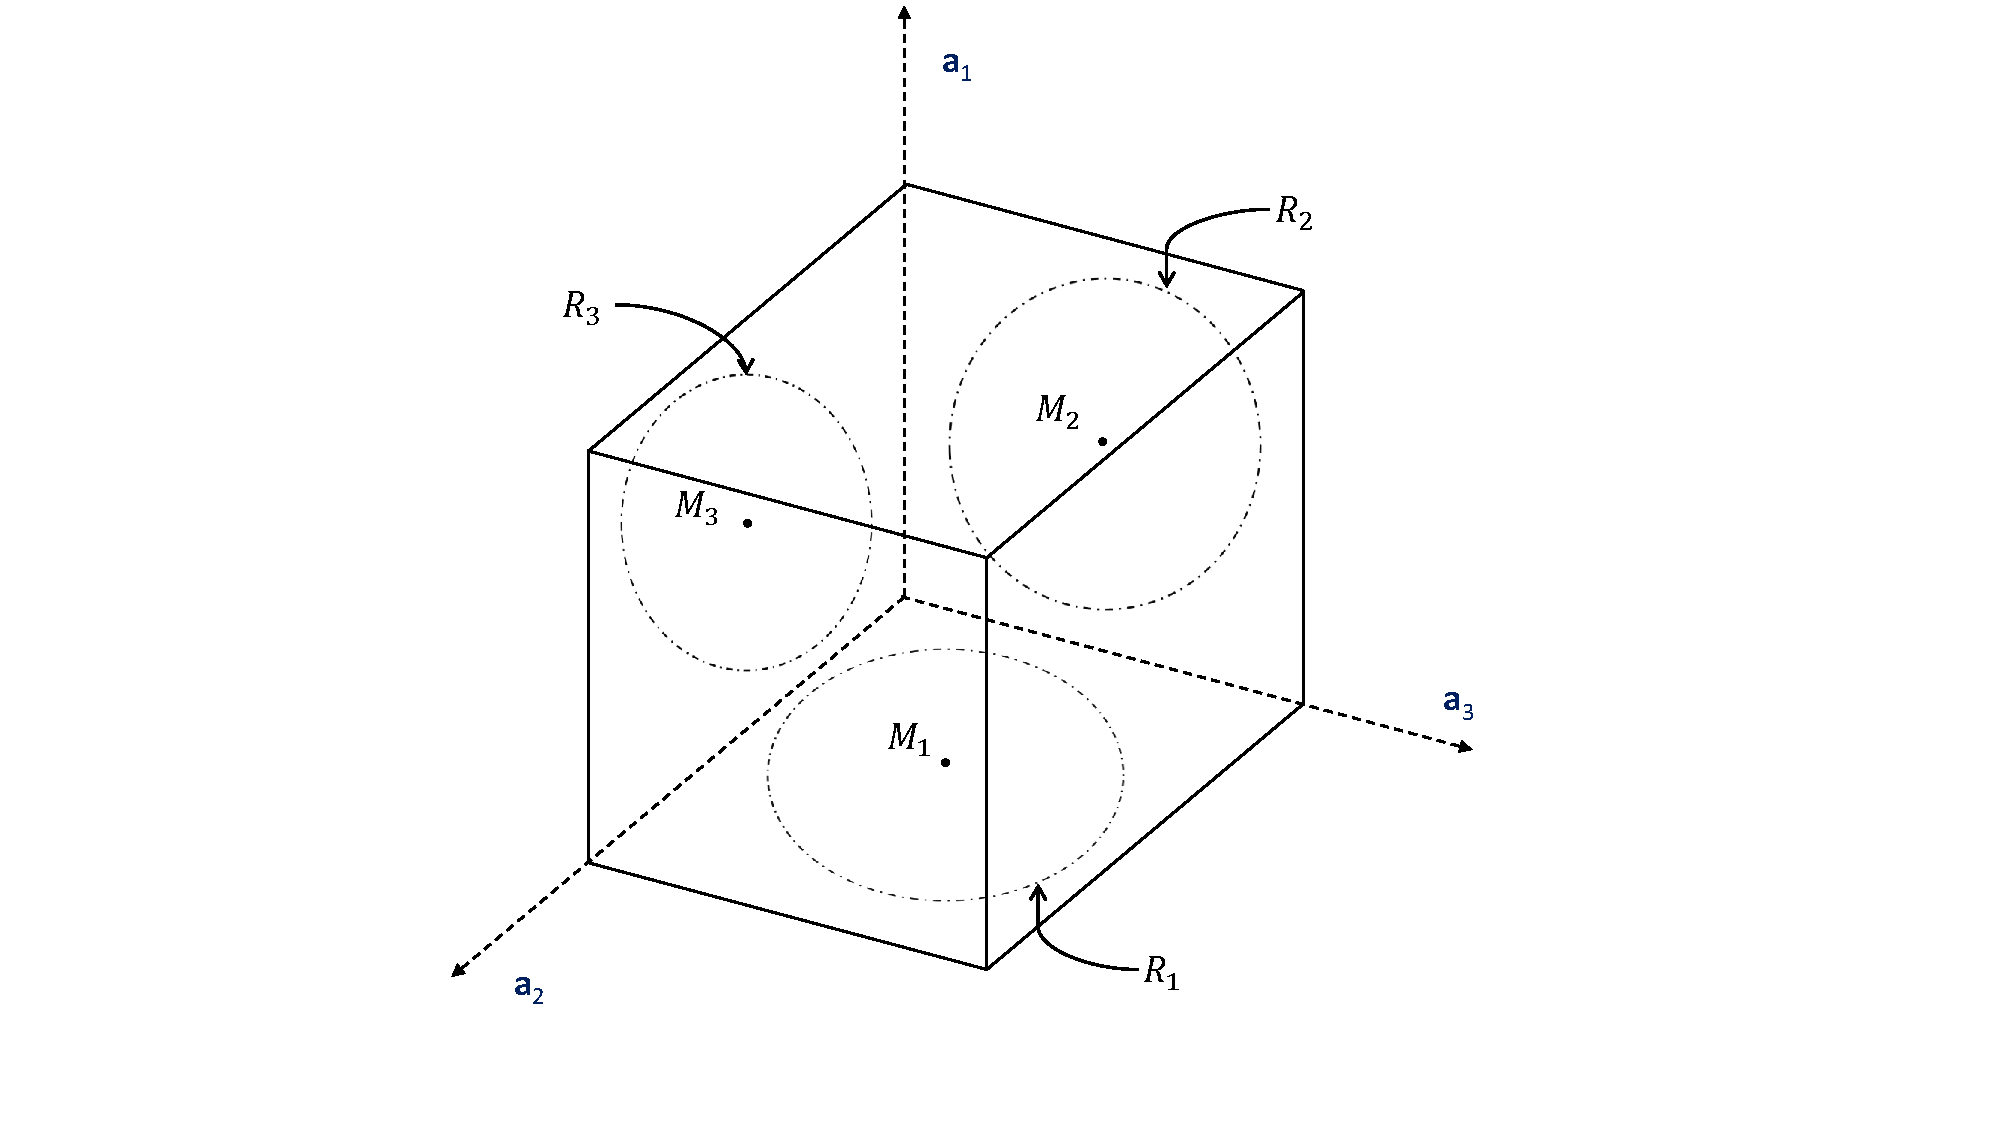
\includegraphics[width=\linewidth, trim={3cm 1.5cm 4cm 0cm}, clip]{5_ModellWuerfel/img/MechAufbau3D}
\caption{Mechanischer Aufbau der Würfelseite, Quelle: eigene Darstellung}
\end{figure}

Durch die Rotation des Würfels um den Winkel $\varphi_1$ in Richtung des Vektors $\bs{a}_1$ entsteht das Hilfsbezugssystem $B$, das durch die Einheitsvektoren $\bs{b}_1$, $\bs{b}_2$ und $\bs{b}_3$ aufgespannt wird.
\begin{equation}
\presuper{A}{\bs{v}} = \presuper{B}{\Big( \pMat{A}{B} \cdot \presuper{A}{\bs{v}}\Big)} = \presuper{B}{\bs{v}} \hspace{35pt} \vert \hspace{15pt} \pMat{A}{B} = \begin{pmatrix}
1 & 0 & 0 \\ 0 & c_{\varphi_1} & s_{\varphi_1} \\ 0 & -s_{\varphi} & c_{\varphi_1}
\end{pmatrix}
\end{equation}
Die Rotation um den Winkel $\varphi_2$ in Richtung des Vektors $\bs{b}_2$ führt zu dem zweiten Hilfsbezugssystem $C$ mit den drei Einheitsvektoren $\bs{c}_1$, $\bs{c}_2$ und $\bs{c}_3$.
\begin{equation}
\presuper{B}{\bs{v}} = \presuper{C}{\Big( \pMat{B}{C} \cdot \presuper{B}{\bs{v}}\Big)} = \presuper{C}{\bs{v}} \hspace{35pt} \vert \hspace{15pt} \pMat{B}{C} = \begin{pmatrix}
c_{\varphi_2} & 0 & -s_{\varphi_2} \\ 0 & 1 & 0 \\ s_{\varphi_2} 0 c_{\varphi_2}
\end{pmatrix}
\end{equation}
Die letzte Rotation des Würfels in Richtung von $\bs{c}_3$ um den Winkel $\varphi_3$ führt zu dem körperfesten Bezugssystem $K$, welches durch die drei Vektoren $\bs{k}_1$, $\bs{k}_2$ und $\bs{k}_3$ definiert ist.
\begin{equation}
\presuper{C}{\bs{v}} = \presuper{K}{\Big( \pMat{C}{K} \cdot \presuper{C}{\bs{v}}\Big)} = \presuper{K}{\bs{v}} \hspace{35pt} \vert \hspace{15pt} \pMat{C}{K} = \begin{pmatrix}
c_{\varphi_3} & s_{\varphi_3} & 0 \\ -s_{\varphi_3} & c_{\varphi_3} & 0 \\ 0 & 0 & 1
\end{pmatrix}
\end{equation}
Hier sei angemerkt, dass es sich bei den Bezugssystem $B$ und $C$ um theoretische Konstrukte handelt, für die kein physisches Gegenstück existiert. Sie werden lediglich als Hilfsmittel zur Beschreibung des Systems verwendet.

Durch die Rotation der Schwungmassen besitzt das System drei weitere Freiheitsgrade, welche von den Winkeln $\psi_1$, $\psi_2$ und $\psi_3$ beschrieben werden. Somit entstehen drei weitere Bezugssysteme, deren Vektorbasen jeweils an den Schwungmassen fixiert sind. Allerdings spielen diese keine weitere Rolle, da es sich bei den Winkeln $\psi_i$ um zyklische Koordinaten handelt. Das heißt, dass der Impuls des Systems nicht von der Ausrichtung der Schwungmassen abhängt. Lediglich die Winkelgeschwindigkeiten $\dot{\psi}_i$ beeinflussen auf Grund der Reibung das System.

Die Position und Ausrichtung des Systems wird von den sechs Winkeln $\varphi_i$ und $\psi_i$ vollständig beschrieben. Deshalb werden diese als generalisierte Koordinaten $q_i$ definiert.
\begin{equation}
q_i = \varphi_i \hspace{35pt} q_j = \psi_i \hspace{35pt} (i=1,2,3; j=4,5,6)
\end{equation}
Mit Hilfe der Bezugssysteme und generalisierten Koordinaten können nun die Winkelgeschwindigkeit des Würfels $\vel{A}{\omega}{K}$ und der Schwungmassen $\vel{A}{\omega}{R_i}$ bestimmt werden. Diese ergeben sich aus der Addition der relativen Rotationsgeschwindigkeiten der Bezugssysteme zueinander.
\begin{equation}
\begin{split}
\vel{A}{\omega}{K} &= \vel{A}{\omega}{B}+\vel{B}{\omega}{C}+\vel{C}{\omega}{K} = \vecBS{A}{\dot{\varphi}_1}{0}{0} + \vecBS{B}{0}{\dot{\varphi}_2}{0} + \vecBS{C}{0}{0}{\dot{\varphi}_3} \\
&= \vecBS{K}
{\dot{\varphi}_2\cdot s_{\varphi_3} + \dot{\varphi}_1 \cdot c_{\varphi_2}\cdot c_{\varphi_3}}
{\dot{\varphi}_2\cdot c_{\varphi_3} - \dot{\varphi}_1 \cdot c_{\varphi_2}\cdot s_{\varphi_3}}
{\dot{\varphi}_3 + \dot{\varphi}_1\cdot s_{\varphi_2}}
\end{split}
\end{equation}
Die Winkelgeschwindigkeiten der Schwungmassen $\vel{K}{\omega}{R_i}$ relativ zu dem Würfel entsprechen der ersten Ableitung der Winkel $\psi_i$. Mit Hilfe des Additionstheorems für Winkelgeschwindigkeiten kann daraus auch die absolute Winkelgeschwindigkeit der Schwungmassen $\vel{A}{\omega}{R_i}$ berechnet werden.
\begin{equation}
\vel{K}{\omega}{R_1} = \vecBS{K}{\dot{\psi}_1}{0}{0} \hspace{35pt}
\vel{K}{\omega}{R_2} = \vecBS{K}{0}{\dot{\psi}_2}{0} \hspace{35pt}
\vel{K}{\omega}{R_3} = \vecBS{K}{0}{0}{\dot{\psi}_3} 
\end{equation}
\begin{equation}
\vel{A}{\omega}{R_i} = \vel{A}{\omega}{K} + \vel{K}{\omega}{R_i} \hspace{35pt} (i=1,2,3)
\end{equation}
Im nächsten Schritt werden die absoluten Geschwindigkeiten der Teilsysteme in Komponenten zerlegt, welche sich aus den generalisierten Geschwindigkeiten $u_i$ und partiellen Geschwindigkeiten $\vel{A}{\omega}{j}_i$ zusammensetzen. Hierfür müssen zu nächst die generalisierten Geschwindigkeiten $u_i$ definiert werden. An dieser Stelle sei erwähnt, dass die Definition der generalisierten Geschwindigkeiten die Form der resultierenden Bewegungsgleichungen stark beeinflusst. Das letztendliche Ziel bei der Wahl der generalisierten Geschwindigkeiten ist es möglichst einfache Bewegungsgleichungen zu erhalten. Dies kann, nach einer Heuristik von Kane, erreicht werden, in dem die generalisierten Geschwindigkeiten so gewählt werden, dass die Geschwindigkeiten der Körper im Intertialsystem auf möglichst einfache Terme reduziert werden können. In diesem Anwendungsfall werden nach diesem Ansatz die folgenden generalisierten Geschwindigkeiten gewählt.
\begin{equation}
\begin{split}
u_1 &= \dot{\varphi}_2\cdot s_{\varphi_3} + \dot{\varphi}_1\cdot c_{\varphi_2}\cdot c_{\varphi_3} \\
u_2 &= \dot{\varphi}_2\cdot c_{\varphi_3} - \dot{\varphi}_1\cdot c_{\varphi_2}\cdot s_{\varphi_3} \\
u_3 &= \dot{\varphi}_3 + \dot{\varphi}_1\cdot s_{\varphi_2} \\
u_4 &= \dot{\varphi}_2\cdot s_{\varphi_3} + \dot{\varphi}_1\cdot c_{\varphi_2}\cdot c_{\varphi_3} + \dot{\psi}_1 \\
u_5 &= \dot{\varphi}_2\cdot c_{\varphi_3} - \dot{\varphi}_1\cdot c_{\varphi_2}\cdot s_{\varphi_3} + \dot{\psi}_2 \\
u_6 &= \dot{\varphi}_3 + \dot{\varphi}_1\cdot s_{\varphi_2} + \dot{\psi}_3
\end{split}
\end{equation}
Mit diesen Definitionen können die Winkelgeschwindigkeiten der Körper im A in die folgende Form gebracht werden.
\begin{equation}
\vel{A}{\omega}{K} = \vecBS{K}{u_1}{u_2}{u_3}, \vel{A}{\omega}{R1} = \vecBS{K}{u_4}{u_2}{u_3}, \vel{A}{\omega}{R2} = \vecBS{K}{u_1}{u_5}{u_3}, \vel{A}{\omega}{R3} = \vecBS{K}{u_1}{u_2}{u_6}
\end{equation}
Die Einführung der generalisierten Geschwindigkeiten führt einerseits zu einem stark vereinfachten Ausdruck der absoluten Winkelgeschwindigkeiten. Andererseits können dadurch auch die partiellen Geschwindigkeiten $\vel{A}{\omega}{j}_i$ in einfachen Termen ausgedrückt werden, wie die folgenden Gleichungen zeigen. Dadurch werden die folgenden Schritte der Modellbildung zunehmend erleichtert. 
\begin{align}
\vel{A}{\omega}{K} &= u_1 \cdot \bs{k}_1 + u_2 \cdot \bs{k}_2 + u_3 \cdot \bs{k}_3 &\rArrow &\vel{A}{\omega}{K}_1 = \bs{k}_1, \vel{A}{\omega}{K}_2 = \bs{k}_2, \vel{A}{\omega}{K}_3 = \bs{k}_3 \\
& & &\vel{A}{\omega}{K}_4 = 0, \vel{A}{\omega}{K}_5 = 0, \vel{A}{\omega}{K}_6 = 0 
\\
\vel{A}{\omega}{R_1} &= u_4 \cdot \bs{k}_1 + u_2 \cdot \bs{k}_2 + u_3 \cdot \bs{k}_3 &\rArrow 
&\vel{A}{\omega}{K}_1 = 0, \vel{A}{\omega}{K}_2 = \bs{k}_2, \vel{A}{\omega}{K}_3 = \bs{k}_3 \\
& & &\vel{A}{\omega}{K}_4 = \bs{k}_1, \vel{A}{\omega}{K}_5 = 0, \vel{A}{\omega}{K}_6 = 0 
\\
\vel{A}{\omega}{R_2} &= u_1 \cdot \bs{k}_1 + u_5 \cdot \bs{k}_2 + u_3 \cdot \bs{k}_3&\rArrow 
&\vel{A}{\omega}{K}_1 = \bs{k}_1, \vel{A}{\omega}{K}_2 = 0, \vel{A}{\omega}{K}_3 = \bs{k}_3 \\
& & &\vel{A}{\omega}{K}_4 = 0, \vel{A}{\omega}{K}_5 = \bs{k}_2, \vel{A}{\omega}{K}_6 = 0 
\\
\vel{A}{\omega}{R_3} &= u_1 \cdot \bs{k}_1 + u_2 \cdot \bs{k}_2 + u_6 \cdot \bs{k}_3&\rArrow 
&\vel{A}{\omega}{K}_1 = \bs{k}_1, \vel{A}{\omega}{K}_2 = \bs{k}_2, \vel{A}{\omega}{K}_3 = 0 \\
& & &\vel{A}{\omega}{K}_4 = 0, \vel{A}{\omega}{K}_5 = 0, \vel{A}{\omega}{K}_6 = \bs{k}_3
\end{align}
Die Unterteilung der absoluten Winkelgeschwindigkeiten in generalisierte und partielle Geschwindigkeiten ermöglicht den Übergang der vektoriellen Rechnung in die skalare. Die generalisierten Geschwindigkeiten geben als skalare Größen den Betrag der Bewegung in die Richtung der jeweiligen Freiheitsgrade wieder. Wobei die partiellen Geschwindigkeiten diese Richtung der Freiheitsgrade als vektorielle Größe mit Bezug auf das körperfeste Bezugssystem $K$ wiedergeben. Dadurch können weitere Vektoren wie z.B. Trägheitsmomente durch die Skalarmultiplikation mit den partiellen Geschwindigkeiten in die Richtung der Freiheitsgrade abgebildet werden.

\subsection{Untersuchung der Kinetik}
Der nächste Schritt besteht darin die Kräfte zu modellieren, die auf den Würfelkörper und die drei Schwungmassen wirken. Aus diesen können im Anschluss mit Hilfe der partiellen Geschwindigkeiten die generalisierten aktiven Kräfte $F_i$ ermittelt werden.
Zunächst sollen die resultierenden Drehmomente $\bs{T}^{Ri/Mi}$ der Schwungmassen $R_i$ um ihren jeweiligen Drehpunkt $M_i$ ermittelt werden. Hierfür muss einerseits das Drehmoment $\bs{T}^{Ri/Mi}_M$ des antreibenden Motors und das verzögernde Reibmoment $\bs{T}^{Ri/Mi}_R$ beachtet werden.
\begin{equation}
\bs{T}^{R1/M1} = \bs{T}^{R1/M1}_M + \bs{T}^{R1/M1}_R = \vecBS{K}{T_{M1}}{0}{0} + \vecBS{K}{-C_{\psi}\cdot (u_4 - u_1)}{0}{0}
\end{equation}
\begin{equation}
\bs{T}^{R2/M2} = \bs{T}^{R2/M2}_M + \bs{T}^{R2/M2}_R = \vecBS{K}{0}{T_{M2}}{0} + \vecBS{K}{0}{-C_{\psi}\cdot (u_5 - u_2)}{0}{0}
\end{equation}
\begin{equation}
\bs{T}^{R3/M3} = \bs{T}^{R3/M3}_M + \bs{T}^{R3/M3}_R = \vecBS{K}{0}{0}{T_{M3}} + \vecBS{K}{0}{0}{-C_{\psi}\cdot (u_6 - u_3)}
\end{equation}
Der Würfelkörper wird einerseits durch das Gravitationsmoment $\bs{T}{K/O}_G$ und die resultierenden Momente der Schwungmassen $\bs{T}{Ri/Mi}$, welche in umgekehrter Richtung auf den Würfel wirken, beeinflusst.
Das Gravitationsmoment hängt von der Gewichtskraft $\bs{G}=\vecBS{A}{-m\cdot g}{0}{0}$ und der Position des Schwerpunktes $bs{c}$ ab.
\begin{equation}
\bs{T}^{K/O}_G = \bs{c} \times \bs{G} = \vecBS{K}{l_C}{l_C}{l_C} \times \vecBS{K}{-m\cdot g \cdot c_{\varphi_2} \cdot c_{\varphi_3}}{-m\cdot g\cdot c_{\varphi_2}\cdot s_{\varphi_3}}{-m\cdot g\cdot s_{\varphi_2}} 
= -m\cdot l_C \cdot g \vecBS{K}{s_{\varphi_2}+c_{\varphi_2}s_{\varphi_3}}
{-s_{\varphi_2}+c_{\varphi_2}c_{\varphi_3}}
{-c_{\varphi_2}c_{\varphi_3} - c_{\varphi_2}\cdot s_{\varphi_3}}
\end{equation}
\begin{equation}
\begin{split}
\bs{T}^{K/O}&=\bs{T}^{K/O}_G - \bs{T}^{R1/M1} - \bs{T}^{R2/M2} - \bs{T}^{R3/M3} \\
&= -m\cdot l_C \cdot g \vecBS{K}{s_{\varphi_2}+c_{\varphi_2}s_{\varphi_3}}
{-s_{\varphi_2}+c_{\varphi_2}c_{\varphi_3}}
{-c_{\varphi_2}c_{\varphi_3} - c_{\varphi_2}\cdot s_{\varphi_3}} - \vecBS{K}{T_{M1}-C_{\psi}(u_4 - u_1)}{T_{M2}-C_{\psi}(u_5 - u_2)}{T_{M3}-C_{\psi}(u_6 - u_3)}
\end{split}
\end{equation}
Im nächsten Schritt können die generalisierten aktiven Kräfte berechnet werden. Dies geschieht durch die Summe der inneren Produkte der resultierenden Drehmomente und der entsprechenden partiellen Geschwindigkeit der Körper. Wenn die partiellen Geschwindigkeiten als die möglichen Bewegungsrichtungen der Körper betrachtet werden, so stellt die Skalarmultiplikation der partiellen Geschwindigkeit und dem resultierenden Drehmoments dessen Abbildung in die Bewegungsrichtung dar. Folglich handelt es sich bei den generalisierten aktiven Kräften um skalare Größen, welche den Einfluss der wirkenden Kräfte und Momente in Richtung der Freiheitsgrade wiedergeben.
\begin{align}
F_1 &= \inProd{\vel{A}{\omega}{K}_1}{\bs{T}^{K/O}} + \sum^3_{i=1} \inProd{\vel{A}{\omega}{Ri}_1}{\bs{T}^{Ri/Mi}} = m\cdot l_C \cdot g (-s_{\varphi_2}-c_{\varphi_2}s_{\varphi_3}) - T_{M1} + C_{\psi}(u_4 - u_1)
\\
F_2 &= \inProd{\vel{A}{\omega}{K}_2}{\bs{T}^{K/O}} + \sum^3_{i=1} \inProd{\vel{A}{\omega}{Ri}_2}{\bs{T}^{Ri/Mi}} = m\cdot l_C \cdot g (s_{\varphi_2}-c_{\varphi_2}c_{\varphi_3})-T_{M2}+C_{\psi}(u_5 - u_2)
\\
F_3 &= \inProd{\vel{A}{\omega}{K}_3}{\bs{T}^{K/O}} + \sum^3_{i=1} \inProd{\vel{A}{\omega}{Ri}_3}{\bs{T}^{Ri/Mi}} = m\cdot l_C \cdot g (c_{\varphi_2}c_{\varphi_3} + c_{\varphi_2}s_{\varphi_3}) - T_{M3} + C_{\psi}(u_6 - u_3)
\\
F_4 &= \inProd{\vel{A}{\omega}{K}_4}{\bs{T}^{K/O}} + \sum^3_{i=1} \inProd{\vel{A}{\omega}{Ri}_4}{\bs{T}^{Ri/Mi}} = T_{M1}-C_{\psi}(u_4 - u_1)
\\
F_5 &= \inProd{\vel{A}{\omega}{K}_5}{\bs{T}^{K/O}} + \sum^3_{i=1} \inProd{\vel{A}{\omega}{Ri}_5}{\bs{T}^{Ri/Mi}} = T_{M2}-C_{\psi}(u_5 - u_2)
\\
F_6 &= \inProd{\vel{A}{\omega}{K}_6}{\bs{T}^{K/O}} + \sum^3_{i=1} \inProd{\vel{A}{\omega}{Ri}_6}{\bs{T}^{Ri/Mi}} = T_{M3}-C_{\psi}(u_6 - u_3)
\end{align}
Neben den aktiven Kräften müssen auch die generalisierten Trägheitskräfte $F^*_i$ ermittelt werden um die Bewegungsgleichungen zu bestimmen. Hierfür werden zunächst die Trägheitsmomente $\bs{T}_*$ der Körper ermittelt werden. Nach Kane gilt für diese Trägheitsmomente der folgende Zusammenhagn.
\begin{equation}
\bs{T}_* = -\bs{\alpha}\cdot \bs{I} - \bs{\omega}\times(\bs{I}\cdot\bs{\omega})
\end{equation}
Wobei $\bs{\alpha}$ und $\bs{\omega}$ die Winkelbeschleunigung- bzw. geschwindigkeit des Körpers und $\bs{I}$ dessen Trägheitstensor bezeichnen. 
Die Winkelgeschwindigkeiten der Körper sind bereits bekannt, die Winkelbeschleunigung ergeben sich durch die Ableitung der Winkelgeschwindigkeiten mit Bezug auf die Vektorbasis von $A$.
\begin{equation}
\vel{A}{\alpha}{K} = \frac{\presuper{A}d}{dt}\vel{A}{\omega}{K}, \vel{A}{\alpha}{R1} = \frac{\presuper{A}d}{dt}\vel{A}{\omega}{R1}, \vel{A}{\alpha}{R2} = \frac{\presuper{A}d}{dt}\vel{A}{\omega}{R2}, \vel{A}{\alpha}{R3} = \frac{\presuper{A}d}{dt}\vel{A}{\omega}{R3}
\end{equation}
Zunächst sollen die Trägheitsmomente $\bs{T}^{Ri/Mi}_*$ der Schwungmassen bestimmt werden. Deren Trägsheitstensoren $\bs{I}^{Ri/Mi}$ im Bezug auf die Drehpunkte $M_i$ wurde, wie in Abschnitt 1 erläutert, mit Hilfe der CAD-Programme ermittelt.
\begin{equation}
\bs{I}^{Ri/Mi} = \begin{pmatrix}
I^{Ri}_{11} & 0 & 0 \\ 0 & I^{Ri}_{22} & 0 \\ 0 & 0 & I^{Ri}_{33}
\end{pmatrix}
\end{equation}
\begin{equation}
\bs{T}^{Ri/Mi}_* = - \vel{A}{\alpha}{Ri} - \vel{A}{\omega}{Ri}\times(\bs{I}^{Ri/Mi} \cdot \vel{A}{\omega}{Ri})
\end{equation}
Der Trägheitstensor $\bs{I}^{K/O}$ des Würfelkörpers um den Punkt $O$ setzt sich aus mehreren Komponenten zusammen. Einerseits wird er durch den Trägheitstensor $\bs{I}^{GH/O}$ des Gehäuses um den Punkt $O$ beeinflusst, dieser Tensor beschreibt die Trägheitseigenschaften des Würfels ohne die Schwungmassen und kann mit Hilfeder CAD-Anwendung ermittelt werden, andererseits beeinflussen die Schwungmassen das Trägheitsmoment des Würfelkörpers. Um diesen Einfluss nachzuvollziehen wird die Bewegung der Schwungmassen in zwei Komponenten zerlegt. Einerseits rotieren die Schwungmassen $R_i$ um die Punkte $M_i$, welche die Schwerpunkte der Schwungmassen sind. Andererseits bewegen sich die Schwerpunkte $M_i$ um den Punkt $O$ und sind bei der Betrachtung der Trägheitseigenschaften dem Würfelkörper zuzuordnen, da sie auf diesem fixiert sind. Hierbei sind sie als Punktmassen mit der Masse $m_R$ zu behandeln. Diese Interpretation entspricht der Aussage des Steiner'schen Satzes.
Somit ist der Trägheitstensor $\bs{I}^{K/O}$ gleich der Summe von $\bs{I}^{GH/O}$ und den Trägheitstensoren der drei Massepunkte $M_i$ mit der Masse $m_R$ um $O$, wobei $\bs{r}_i$ den Ortsvektor des Punktes $M_i$ beschreibt.
\begin{equation}
\bs{I}^{K/O} = \bs{I}^{GH/O} + \sum^3_{i=1}m_R(\inProd{\bs{r}_i}{\bs{r}_i}-\bs{r}_i\otimes\bs{r}_i)
\end{equation}
\begin{equation}
\bs{T}^{K/O}_* = - \vel{A}{\alpha}{K}\cdot\bs{I}^{K/O} - \vel{A}{\omega}{K}\times(\bs{I}^{K/O}\cdot \vel{A}{\omega}{K})
\end{equation}
Prinzipiell können nun analog zu den generalisierten aktiven Kräfte durch die Skalarmultiplikation mit den partiellen Geschwindigkeiten die generalisierten Trägheitskräfte berechnet werden. Allerdings handelt es sich bei Trägheitsmomenten um recht komplexe und insbesondere stark nichtlinearen Termen. Diese führen wiederum auf schwer nachzuvollziehende Bewegungsgleichungen. Außerdem werden für die Transformation in eine Zustandsraumdarstellung lineare Differentialgleichungen vorliegen. Für diesen Fall schlägt Kane eine vorzeitige Linearisierung vor. Das heißt an Stelle die vollständigen, nicht linearen Bewegungsgleichungen zu bestimmen und anschließend zu linearisieren, werden bereits die generalisierten  Geschwindigkeiten $\hat{\bs{\omega}}$, sowie die resultierenden Dreh- und Trägheitsmomente $\hat{F}_i$ und $\hat{F}^*_i$ linearisiert und daraus die linearen Bewegungsgleichungen bestimmt.
Hierfür muss zunächst der Arbeitspunkt des Systems bestimmt werden, welcher der balancieren Position entspricht. Die Winkel $\varphi_i$ müssen folglich so gewählt werden, dass der Ortsvektor des Schwerpunktes $\bs{c}$ aus Perspektive des Inertialsystems lediglich eine Komponente in Richtung von $\bs{a}_1$ besitzt.
\begin{equation}
\vecBS{A}{\vert \bs{c} \vert}{0}{0} \overset{!}= \pMat{K}{A}\cdot \vecBS{K}{l_C}{l_C}{l_C} \rArrow \varphi_{10} = 0, \hspace{10pt} \varphi_{20} =-2\cdot atan(\sqrt{2}-\sqrt{3})\approx0.62, \hspace{10pt} \varphi_{30}=\frac{-\pi}{4}
\end{equation}
\begin{equation}
\hat{\varphi}_i = \varphi_{i0} + \bar{\varphi}_i
\end{equation}
In dem Gleichgewichtspunkt verschwinden die Winkelgeschwindigkeiten des Systems, folglich gilt für die generalisierten Geschwindigkeiten im Arbeitspunkt $u_{i0} = 0$.
\begin{equation}
\begin{split}
\hat{u}_1 &= \dot{\varphi}_2\cdot s_{\varphi_{30}} + \dot{\varphi}_1\cdot c_{\varphi_{20}}c_{\varphi_{30}} \\
\hat{u}_2 &= \dot{\varphi}_2\cdot c_{\varphi_{30}} - \dot{\varphi}_1\cdot c_{\varphi_{20}} s_{\varphi_{30}} \\
\hat{u}_3 &= \dot{\varphi}_3 + \dot{\varphi}_1\cdot s_{\varphi_{20}} \\
\hat{u}_4 &= \dot{\varphi}_2\cdot s_{\varphi_{30}} + \dot{\varphi}_1\cdot c_{\varphi_{20}} c_{\varphi_{30}} + \dot{\psi}_1 \\
\hat{u}_5 &= \dot{\varphi}_2\cdot c_{\varphi_{30}} - \dot{\varphi}_1\cdot c_{\varphi_{20}}s_{\varphi_{30}} + \dot{\psi}_2 \\
\hat{u}_6 &= \dot{\varphi}_3 + \dot{\varphi}_1\cdot s_{\varphi_{20}} + \dot{\psi}_3
\end{split}
\end{equation}
\begin{equation}
\vel{A}{\hat{\omega}}{K} = \vecBS{K}{\hat{u}_1}{\hat{u}_2}{\hat{u}_3}, \hspace{10pt} \vel{A}{\hat{\omega}}{R1} = \vecBS{K}{\hat{u}_4}{\hat{u}_2}{\hat{u}_3}, \hspace{10pt}
\vel{A}{\hat{\omega}}{R2} = \vecBS{K}{\hat{u}_1}{\hat{u}_5}{\hat{u}_3}, \hspace{10pt}
\vel{A}{\hat{\omega}}{R3} = \vecBS{K}{\hat{u}_1}{\hat{u}_2}{\hat{u}_6}
\end{equation}
Insbesondere die Winkelbeschleunigungen werden durch die linearisierten Winkelgeschwindigkeiten stark vereinfacht.
\begin{equation}
\vel{A}{\hat{\alpha}}{K} = \frac{\presuper{A}d}{dt}\vel{A}{\hat{\omega}}{K} = \vecBS{K}{\ddot{\varphi}_2\cdot s_{\varphi_{30}} + \ddot{\varphi}_1\cdot c_{\varphi_{20}}c_{\varphi_{30}}}{\ddot{\varphi}_2\cdot c_{\varphi_{30}} - \ddot{\varphi}_1\cdot c_{\varphi_{20}} s_{\varphi_{30}}}{\ddot{\varphi}_3 + \ddot{\varphi}_1\cdot s_{\varphi_{20}}} = \vecBS{K}{\hat{\dot{u}}_1}{\hat{\dot{u}}_2}{\hat{\dot{u}}_3}
\end{equation}
\begin{equation}
\vel{A}{\hat{\alpha}}{R1} = \frac{\presuper{A}d}{dt}\vel{A}{\hat{\omega}}{R1} = \vecBS{K}{\ddot{\varphi}_2\cdot s_{\varphi_{30}} + \ddot{\varphi}_1\cdot c_{\varphi_{20}}c_{\varphi_{30}}+\ddot{\psi}_1}{\ddot{\varphi}_2\cdot c_{\varphi_{30}} - \ddot{\varphi}_1\cdot c_{\varphi_{20}} s_{\varphi_{30}}}{\ddot{\varphi}_3 + \ddot{\varphi}_1\cdot s_{\varphi_{20}}} = \vecBS{K}{\hat{\dot{u}}_4}{\hat{\dot{u}}_2}{\hat{\dot{u}}_3}
\end{equation}
\begin{equation}
\vel{A}{\hat{\alpha}}{R2} = \frac{\presuper{A}d}{dt}\vel{A}{\hat{\omega}}{R2} = \vecBS{K}{\ddot{\varphi}_2\cdot s_{\varphi_{30}} + \ddot{\varphi}_1\cdot c_{\varphi_{20}}c_{\varphi_{30}}}{\ddot{\varphi}_2\cdot c_{\varphi_{30}} - \ddot{\varphi}_1\cdot c_{\varphi_{20}} s_{\varphi_{30}} + \ddot{\psi}_2}{\ddot{\varphi}_3 + \ddot{\varphi}_1\cdot s_{\varphi_{20}}} = \vecBS{K}{\hat{\dot{u}}_1}{\hat{\dot{u}}_5}{\hat{\dot{u}}_3}
\end{equation}
\begin{equation}
\vel{A}{\hat{\alpha}}{K} = \frac{\presuper{A}d}{dt}\vel{A}{\hat{\omega}}{K} = \vecBS{K}{\ddot{\varphi}_2\cdot s_{\varphi_{30}} + \ddot{\varphi}_1\cdot c_{\varphi_{20}}c_{\varphi_{30}}}{\ddot{\varphi}_2\cdot c_{\varphi_{30}} - \ddot{\varphi}_1\cdot c_{\varphi_{20}} s_{\varphi_{30}}}{\ddot{\varphi}_3 + \ddot{\varphi}_1\cdot s_{\varphi_{20}} + \ddot{\psi}_3} = \vecBS{K}{\hat{\dot{u}}_1}{\hat{\dot{u}}_2}{\hat{\dot{u}}_6}
\end{equation}
Somit können nun die linearisierten Trägheitsmomente berechnet werden, wobei der zweite Term auf Grund der Linearisierung entfällt.
\begin{equation}
\hat{\bs{T}}^{R1/M1}_* = -\vel{A}{\hat{\alpha}}{R1}\cdot \bs{I}^{R1/M1} = \vecBS{K}{-\hat{\dot{u}}_4\cdot I^{R1}_{11}}{-\hat{\dot{u}}_2\cdot I^{R1}_{22}}{-\hat{\dot{u}}_3\cdot I^{R3}_{33}}
\end{equation}
\begin{equation}
\hat{\bs{T}}^{R2/M2}_* = -\vel{A}{\hat{\alpha}}{R2}\cdot \bs{I}^{R2/M2} = \vecBS{K}{-\hat{\dot{u}}_1\cdot I^{R2}_{11}}{-\hat{\dot{u}}_5\cdot I^{R2}_{22}}{-\hat{\dot{u}}_3\cdot I^{R2}_{33}}
\end{equation}
\begin{equation}
\hat{\bs{T}}^{R3/M3}_* = -\vel{A}{\hat{\alpha}}{R3}\cdot \bs{I}^{R3/M3} = \vecBS{K}{-\hat{\dot{u}}_1\cdot I^{R3}_{11}}{-\hat{\dot{u}}_2\cdot I^{R3}_{22}}{-\hat{\dot{u}}_6\cdot I^{R3}_{33}}
\end{equation}
Bei der Berechnung des Trägheitsmomentes $\hat{\bs{T}}^{K/O}$ muss beachtet werden, dass die Devitationsmomente des Tensors $\bs{I}^{K/O}$ nicht verschwinden und deshalb ein etwas komplexerer Ausdruck für das Trägheitsmoment resultiert.
\begin{equation}
\hat{\bs{T}}^{K/O}_* = -\vel{A}{\hat{\alpha}}{K}\cdot \bs{I}^{K/O} = -\vecBS{K}
{\hat{\dot{u}}_1\cdot I^{K}_{11} + \hat{\dot{u}}_2\cdot I^{K}_{21} + \hat{\dot{u}}_3\cdot I^{K}_{31}}
{\hat{\dot{u}}_1\cdot I^{K}_{12} + \hat{\dot{u}}_2\cdot I^{K}_{22} + \hat{\dot{u}}_3\cdot I^{K}_{32}}
{\hat{\dot{u}}_1\cdot I^{K}_{13} + \hat{\dot{u}}_2\cdot I^{K}_{23} + \hat{\dot{u}}_3\cdot I^{K}_{33}}
\end{equation}
Nun können nun mit Hilfe der partiellen Geschwindigkeiten, welche durch die Linearisierung nicht beeinflusst werden, die generalisierten Trägheitskräfte $\hat{F}^*_i$ berechnet werden.
\begin{align}
\hat{F}^*_1 &= \inProd{\hat{\bs{T}}^{K/O}_*}{\vel{A}{\omega}{K}_1} + \sum^3_{i=1}\inProd{\hat{\bs{T}}^{Ri/Mi}_*}{\vel{A}{\omega}{Ri}_1} = -\hat{\dot{u}}_1(I^K_{11}+I^{R2}_{11}+I^{R3}_{11}) - \hat{\dot{u}}_2\cdot I^{K}_{21} - \hat{\dot{u}}_3\cdot I^{K}_{31}
\\
\hat{F}^*_2 &= \inProd{\hat{\bs{T}}^{K/O}_*}{\vel{A}{\omega}{K}_2} + \sum^3_{i=1}\inProd{\hat{\bs{T}}^{Ri/Mi}_*}{\vel{A}{\omega}{Ri}_2} = -\hat{\dot{u}}_1\cdot I^{K}_{12} - \hat{\dot{u}}_2(I^{K}_{22}+I^{R1}_{22}+I^{R3}_{33}) - \hat{\dot{u}}_3\cdot I^{K}_{13} 
\\
\hat{F}^*_3 &= \inProd{\hat{\bs{T}}^{K/O}_*}{\vel{A}{\omega}{K}_3} + \sum^3_{i=1}\inProd{\hat{\bs{T}}^{Ri/Mi}_*}{\vel{A}{\omega}{Ri}_3} = -\hat{\dot{u}}_1\cdot I^{K}_{13} - \hat{\dot{u}}_2\cdot I^{K}_{23} - \hat{\dot{u}}_3(I^{K}_{33}+I^{R1}_{33}+I^{R2}_{33})
\\
\hat{F}^*_4 &= \inProd{\hat{\bs{T}}^{K/O}_*}{\vel{A}{\omega}{K}_4} + \sum^3_{i=1}\inProd{\hat{\bs{T}}^{Ri/Mi}_*}{\vel{A}{\omega}{Ri}_4} = -\hat{\dot{u}}_4\cdot I^{R1}_{11}
\\
\hat{F}^*_5 &= \inProd{\hat{\bs{T}}^{K/O}_*}{\vel{A}{\omega}{K}_5} + \sum^3_{i=1}\inProd{\hat{\bs{T}}^{Ri/Mi}_*}{\vel{A}{\omega}{Ri}_5} = -\hat{\dot{u}}_5\cdot I^{R2}_{22}
\\
\hat{F}^*_6 &= \inProd{\hat{\bs{T}}^{K/O}_*}{\vel{A}{\omega}{K}_6} + \sum^3_{i=1}\inProd{\hat{\bs{T}}^{Ri/Mi}_*}{\vel{A}{\omega}{Ri}_6} = -\hat{\dot{u}}_6\cdot I^{R3}_{33}
\end{align}
Zuletzt müssen nur noch die generalisierten aktiven Kräfte linearisiert werden um mit Hilfe von Kanes Gleichungen die Bewegungsgleichungen zu ermitteln. Hierbei muss lediglich das Gravitationsmoment $\bs{T}^{K/O}_G$ linearisiert werden, da die restlichen Momente bereits in linearer Form vorliegen.
\begin{equation}
\hat{\bs{T}}^{K/O}_G = -m\cdot g\cdot l_C \vecBS{K}
{(c_{\varphi_{20}}-s_{\varphi_{20}}c_{\varphi_{30}})\bar{\varphi}_2 + c_{\varphi_{20}}c_{\varphi_{30}}\bar{\varphi}_3}
{(-c_{\varphi_{20}}-s_{\varphi_{20}}c_{\varphi_{30}})\bar{\varphi}_2 - c_{\varphi_{20}}s_{\varphi_{30}}\bar{\varphi}_3 }
{(s_{\varphi_{20}}s_{\varphi_{30}}+s_{\varphi_{20}}c_{\varphi_{30}})\bar{\varphi}_2 + (c_{\varphi_{20}}s_{\varphi_{30}} - c_{\varphi_{20}}c_{\varphi_{30}})\bar{\varphi}_3}
\end{equation}
\begin{align}
\hat{F}_1 &= -m\cdot g\cdot l_C (c_{\varphi_{20}}-s_{\varphi_{20}}c_{\varphi_{30}})\bar{\varphi}_2 + c_{\varphi_{20}}c_{\varphi_{30}}\bar{\varphi}_3 - T_{M1} + C_{\psi}(\hat{u}_4 - \hat{u}_1) 
\\
\hat{F}_1 &= -m\cdot g\cdot l_C [(-c_{\varphi_{20}}-s_{\varphi_{20}}c_{\varphi_{30}})\bar{\varphi}_2 - c_{\varphi_{20}}s_{\varphi_{30}}\bar{\varphi}_3 ] - T_{M2} + C_{\psi}(\hat{u}_5 - \hat{u}_2)
\\
\hat{F}_3 &= -m\cdot g\cdot l_C [(s_{\varphi_{20}}s_{\varphi_{30}}+s_{\varphi_{20}}c_{\varphi_{30}})\bar{\varphi}_2 + (c_{\varphi_{20}}s_{\varphi_{30}} - c_{\varphi_{20}}c_{\varphi_{30}})\bar{\varphi}_3] - T_{M3} + C_{\psi}(\hat{u}_6 - \hat{u}_3)
\\
\hat{F}_4 &= T_{M1} - C_{\psi}(\hat{u}_4 - \hat{u}_1)
\\
\hat{F}_5 &= T_{M2} - C_{\psi}(\hat{u}_5 - \hat{u}_2)
\\
\hat{F}_6 &= T_{M3} - C_{\psi}(\hat{u}_6 - \hat{u}_3)
\end{align}
An dieser Stelle können nun prinzipiell nach Kanes Gleichung
\begin{equation}
F_i + F^*_i = 0
\end{equation}
die Bewegungsgleichungen bestimmt werden. Allerdings wird in diesem Fall eine vektorielle Vorgehensweise gewählt, welche einen eleganten Weg zur gewünschten Zustandsraumdarstellung darstellt. Zunächst werden die folgenden Definition getroffen.
\begin{equation}
\bs{u}_K \equiv \begin{bmatrix} \hat{u}_1 \\ \hat{u}_2 \\ \hat{u}_3 \end{bmatrix}
\hspace{35pt}
\bs{u}_R \equiv \begin{bmatrix} \hat{u}_4 \\ \hat{u}_5 \\ \hat{u}_6 \end{bmatrix}
\end{equation}
\begin{equation}
\begin{split}
\bs{F}^*_K &= \begin{bmatrix}-F^*_1 \\ -F^*_2 \\ -F^*_3\end{bmatrix} = 
\begin{bmatrix}
\hat{\dot{u}}_1(I^K_{11}+I^{R2}_{11}+I^{R3}_{11}) + \hat{\dot{u}}_2\cdot I^{K}_{21} + \hat{\dot{u}}_3\cdot I^{K}_{31}
\\
\hat{\dot{u}}_1\cdot I^{K}_{12} + \hat{\dot{u}}_2(I^{K}_{22}+I^{R1}_{22}+I^{R3}_{33}) + \hat{\dot{u}}_3\cdot I^{K}_{13} 
\\
\hat{\dot{u}}_1\cdot I^{K}_{13} + \hat{\dot{u}}_2\cdot I^{K}_{23} + \hat{\dot{u}}_3(I^{K}_{33}+I^{R1}_{33}+I^{R2}_{33})
\end{bmatrix} \\
&= 
\underbrace{
\begin{bmatrix}
I^K_{11}+I^{R1}_{11}+I^{R2}_{11} & I^K_{21} & I^K_{31} \\
I^K_{12} & I^K_{22}+I^{R1}_{22}+I^{R3}_{22} & I^K_{32} \\
I^K_{13} & I^K_{23} & I^K_{33}+I^{R1}_{33}+I^{R2}_{33}
\end{bmatrix}}_{\equiv \bs{I}_K} \cdot \underbrace{\begin{bmatrix}
\hat{\dot{u}}_1 \\ \hat{\dot{u}}_2 \\ \hat{\dot{u}}_3
\end{bmatrix}}_{\equiv \bs{\dot{u}}_K}
\end{split}
\end{equation} 
\begin{equation}
\begin{split}
\bs{F}^*_R &= \begin{bmatrix}-F^*_4 \\ -F^*_5 \\ -F^*_6 \end{bmatrix} = 
\begin{bmatrix}
\hat{\dot{u}}_4 \cdot I^{R1}_{11} \\ \hat{\dot{u}}_5\cdot I^{R2}_{22} \\ \hat{\dot{u}}_6\cdot I^{R3}_{33}
\end{bmatrix} = \underbrace{\begin{bmatrix}
I^{R1}_11 & 0 & 0 \\ 0 & I^{R2}_{22} & 0 \\ 0 & 0 & I^{R3}_{33}
\end{bmatrix}}_{\equiv \bs{I}_R} \cdot \underbrace{\begin{bmatrix}
\hat{\dot{u}}_4 \\ \hat{\dot{u}}_5 \\ \hat{\dot{u}}_6
\end{bmatrix}}_{\equiv \bs{\dot{u}}_R}
\end{split}
\end{equation}
\begin{equation}
\begin{split}
\bs{F}_K &= \vecBS{K}{m\cdot l_C}{m\cdot l_C}{m\cdot l_C} \times \underbrace{\vecBS{K}{-g\cdot c_{\varphi_{20}}c_{\varphi_{30}}}{g\cdot c_{\varphi_{20}}s_{\varphi_{30}}}{-g\cdot s_{\varphi_{20}}}}_{\equiv \bs{g}} + C_{\psi}\cdot \begin{bmatrix}
\hat{u}_4 - \hat{u}_1 \\ \hat{u}_5 - \hat{u}_2 \\ \hat{u}_6 - \hat{u}_3
\end{bmatrix} - \underbrace{\begin{bmatrix}
T_{M1} \\ T_{M2} \\ T_{M3}
\end{bmatrix}}_{\equiv \bs{T}_M}
\\
&= \underbrace{\begin{bmatrix}
0 & -m\cdot l_C & m\cdot l_C \\ m\cdot l_C & 0 & -m\cdot l_C \\ -m\cdot l_C & m\cdot l_C & 0
\end{bmatrix}}_{\equiv \bs{G_{LA}}} \cdot \bs{g} + C_{\psi} \cdot \bs{u}_R - C_{\psi} \cdot \bs{u}_K  - \bs{T}_M
\end{split}
\end{equation}
\begin{equation}
\bs{F}_R = \begin{bmatrix} F_4 \\ F_5 \\ F_6 \end{bmatrix} = \sum^3_{i=1} \presuper{K}{\bs{T}^{Ri/Mi}} = \begin{bmatrix}
T_{M1} \\ T_{M2} \\ T_{M3}
\end{bmatrix} - C_{\psi}\cdot \begin{bmatrix}
\hat{u}_4 - \hat{u}_1 \\ \hat{u}_5 - \hat{u}_2 \\ \hat{u}_6 - \hat{u}_3
\end{bmatrix}
\end{equation}
Nach Kanes Gleichung gilt $F_i=-F^*_i$, somit muss auch $\bs{F}_K=\bs{F}^*_K$ und $\bs{F}_R=\bs{F}^*_R$ gelten. Daraus resultieren die folgenden Zusammenhänge.
\begin{align}
\label{eq_ZRD3D_zeile2}
\bs{\dot{u}}_K &= \bs{I}^{-1}_K \cdot \bs{F}^*_K = \bs{I}^{-1}_K \cdot \bs{F}_K 
= \bs{I}^{-1}_K \cdot \bs{G}_{LA}\cdot \bs{g} - C_{\psi}\cdot \bs{I}^{-1}_K \cdot \bs{u}_K + C_{\psi}\cdot \bs{I}^{-1}_K \cdot \bs{u}_R - \bs{I}^{-1}_K \cdot \bs{T}_M
\\
\label{eq_ZRD3D_zeile3}
\bs{\dot{u}}_R &= \bs{I}^{-1}_R \cdot \bs{F}^*_R = \bs{I}^{-1}_R \cdot \bs{F}_K =
 C_{\psi}\cdot \bs{I}^{-1}_R \cdot \bs{u}_K - C_{\psi}\cdot \bs{I}^{-1}_R \cdot \bs{u}_R + \bs{I}^{-1}_R \cdot \bs{T}_M
\end{align}
Wenn nun ein Zustandsvektor $\bs{x} \equiv \begin{bmatrix} \bs{g} & \bs{u}_K & \bs{u}_R\end{bmatrix}^T$ und ein Eingangsvektor $\bs{u} \equiv \bs{T}_M$ definiert werden, geben die obigen Gleichungen bereits zwei Drittel der gesuchten Zustandsraumdarstellung wieder. Der letzte Teil ergibt sich durch die Ableitung des Gravitationsmomentes $\bs{g}$ in Bezug auf das körperfeste System $K$. Nach Kane gilt für einen Vektor $\bs{p}$ der in einem Bezugssystem $B$ fixiert ist, welches sich mit der Winkelgeschwindigkeit $\vel{A}{\omega}{B}$ in dem Bezugssystem $A$ bewegt:
\begin{equation}
\frac{\presuper{A}{d}\bs{p}}{dt} = \vel{A}{\omega}{B} \times \bs{p}
\end{equation}
Dieser Zusammenhang kann genutzt werden um die Ableitung von $\bs{g}$ mit Respekt zu $K$ zu bestimmen. Und zwar ist der Gravitationsvektor $\bs{g}$ im Intertialsystem $A$ fixiert. Des weiteren bewegt sich das Intertialsystem $A$ aus Perspektive des Würfelkörpers mit der Geschwindigkeit $\vel{K}{\omega}{A}$, welche gleich der richtungsinvertierten Winkelgeschwindigkeit $\vel{A}{\omega}{K}$ des Würfels ist. Somit gilt für die erste Ableitung von $\bs{g}$ in $K$:
\begin{equation}
\label{eq_ZRD3D_zeile1}
\begin{split}
\frac{\presuper{K}{d \bs{g}}}{dt} &= \vel{K}{\omega}{A} \times \bs{g} = -\vel{A}{\omega}{A} \times \bs{g} = \vecBS{K}{-g\cdot c_{\varphi_{20}}c_{\varphi_{30}}}{g\cdot c_{\varphi_{20}}s_{\varphi_{30}}}{-g\cdot s_{\varphi_{20}}} \times \vecBS{K}{\hat{u}_1}{\hat{u}_2}{\hat{u}_3} 
\\
&= \underbrace{\begin{bmatrix}
0 & g\cdot s_{\varphi_{20}} & g\cdot c_{\varphi_{20}}s_{\varphi_{30}} \\
-g\cdot s_{\varphi_{20}} & 0 & g\cdot c_{\varphi_{20}}c_{\varphi_{30}} \\
-g\cdot c_{\varphi_{20}}s_{\varphi_{30}} & -g\cdot c_{\varphi_{20}}c_{\varphi_{30}} & 0
\end{bmatrix}}_{\bs{\dot{g}}_{LA}} \cdot \bs{u}_K
\end{split}
\end{equation}
Diese Umformung macht sich analog zu der Berechnung von $\bs{G}_{LA}$ zu Nutze, dass Kreuzprodukte als lineare Abbildung dargestellt werden können. 
Nun können die Gleichungen (\ref{eq_ZRD3D_zeile1}), (\ref{eq_ZRD3D_zeile2}) und (\ref{eq_ZRD3D_zeile3}) zu einer Zustandsraumdarstellung zusammengeführt werden.
\begin{equation}
\underbrace{\begin{bmatrix} \dot{\bs{g}} \\ \dot{\bs{u}}_K \\ \dot{\bs{u}}_R \end{bmatrix}}_{\equiv \dot{\bs{x}}} 
= 
\underbrace{\begin{bmatrix}
0^{3x3} & \bs{\dot{g}}_{LA} & 0^{3x3} \\
\bs{I}^{-1}_K \cdot \bs{G}_{LA} & -C_{\psi}\cdot \bs{I}^{-1}_K & C_{\psi}\cdot \bs{I}^{-1}_K \\
0^{3x3} & C_{\psi}\cdot \bs{I}^{-1}_R & -C_{\psi}\cdot \bs{I}^{-1}_R
\end{bmatrix}}_{\equiv \bs{A}}
\cdot
\underbrace{\begin{bmatrix}\bs{g} \\ \bs{u}_K \\ \bs{u}_R\end{bmatrix}}_{\equiv \bs{x}}
+
\underbrace{\begin{bmatrix}
0^{3x3} \\ -\bs{I}^{-1}_K \\ \bs{I}^{-1}_R
\end{bmatrix}}_{\equiv \bs{B}}
\cdot
\underbrace{\begin{bmatrix}
T_{M1} \\ T_{M2} \\ T_{M3}
\end{bmatrix}}_{\equiv \bs{u}}
\end{equation}